\documentclass[25pt, a0paper, portrait]{tikzposter}
\usepackage[T1]{fontenc}
\renewcommand*\familydefault{\sfdefault}
\usepackage{sfmath}
\usepackage{amsmath}
\usepackage{lipsum}
\usepackage[compress]{cite}

\newcommand{\CORE}{The CORE collaboration}
\newcommand{\PLANCK}{The Planck collaboration}
\newcommand{\prd}{PRD}
\newcommand{\prr}{PRR}
\newcommand{\mnras}{MNRAS}
\newcommand{\jcap}{JCAP}
\newcommand{\jmap}{JMAP}
\newcommand{\joss}{JOSS}
\newcommand{\pasa}{PASA}
\newcommand{\aap}{A\&A}
\newcommand{\prl}{PRL}
\newcommand{\arxiv}{arXiv}

\definecolor{C0}{HTML}{1f77b4}
\definecolor{C1}{HTML}{ff7f0e}
\definecolor{C2}{HTML}{2ca02c}
\definecolor{C3}{HTML}{d62728}
\definecolor{C4}{HTML}{9467bd}
\definecolor{C5}{HTML}{8c564b}
\definecolor{C6}{HTML}{e377c2}
\definecolor{C7}{HTML}{7f7f7f}
\definecolor{C8}{HTML}{bcbd22}
\definecolor{C9}{HTML}{17becf}
\newcommand\C[2][1]{\textcolor{C#1}{#2}}

% Packages added by me
\usepackage[inline]{enumitem}
\makeatletter
\usepackage{tcolorbox}
\usepackage{graphicx}
\usepackage{wrapfig}


\makeatletter
\renewcommand\TP@maketitle{%
    \centering
    \vspace{-30pt}
    %
\includegraphics[height=0.11\textwidth]{kicc.png}\hfill
    \hspace{-1cm}
    \begin{minipage}[b]{0.17\linewidth}
        \centering
        
\includegraphics[height=0.5\textwidth]{kicc.png}
        
        
\includegraphics[height=0.2\textwidth]{dirac.png}\hfill
    \end{minipage}%
    %
\includegraphics[height=0.04\textwidth]{dirac.png}\hfill
    \begin{minipage}[b]{0.7\linewidth}
        \centering
        \color{titlefgcolor}
        {\Huge \texttt{unimpeded}: A universal parameter estimation, model comparison and tension quantification distributed over every dataset \par}
        \vspace*{1em}
        {\huge \@author \par}
        \vspace*{1em}
        {\LARGE \@institute}
    \end{minipage}%
    \hfill
\includegraphics[height=0.11\textwidth]{cambridge-cropped.pdf}
}
\makeatother

%\title{unimpeded: A universal model comparison and parameter estimation \\ distributed over every dataset}
\author{Dily Duan Yi Ong <dlo26@cam.ac.uk>, Will Handley <wh260@cam.ac.uk>}
\institute{University of Cambridge $\cdot$ Kavli Institute for Cosmology $\cdot$ Cavendish Laboratory}
%\usetheme{Default}
%\usetheme{Rays}
%\usetheme{Basic}
%\usetheme{Simple}
\usetheme{Envelope}
%\usetheme{Wave}
%\usetheme{Board}
%\usetheme{Autumn}
%\usetheme{Desert}

\tikzposterlatexaffectionproofoff{}

\let\oldbibliography\thebibliography
\renewcommand{\thebibliography}[1]{\oldbibliography{#1}
\setlength{\itemsep}{-5pt}} %Reducing spacing in the bibliography.

\pdfinclusioncopyfonts=1 % Fix fonts on non-linux machines

\usepackage{xcolor}
\definecolor{C0}{HTML}{1f77b4}
\definecolor{C1}{HTML}{ff7f0e}
\definecolor{C2}{HTML}{2ca02c}
\definecolor{C3}{HTML}{d62728}
\definecolor{C4}{HTML}{9467bd}
\definecolor{C5}{HTML}{8c564b}
\definecolor{C6}{HTML}{e377c2}
\definecolor{C7}{HTML}{7f7f7f}
\definecolor{C8}{HTML}{bcbd22}
\definecolor{C9}{HTML}{17becf}
%\newcommand\C[2][1]{\textcolor{C#1}{#2}}


%\usecolorstyle[colorOne=blue, colorTwo=gray, colorThree=green]{Default}
%\usecolorpalette{BlueGrayOrange}
%\usecolorstyle[colorOne=blue]{mystyle}
%\colorlet{backgroundcolor}{C1}

%% Background Colors
\colorlet{backgroundcolor}{C0!50!white}
\colorlet{framecolor}{black}
%% Title Colors
\colorlet{titlefgcolor}{white}
\colorlet{titlebgcolor}{C0}
%% Block Colors
\colorlet{blocktitlebgcolor}{C0}
\colorlet{blocktitlefgcolor}{white}
\colorlet{blockbodybgcolor}{white}
\colorlet{blockbodyfgcolor}{black}
%% Innerblock Colors
\colorlet{innerblocktitlebgcolor}{C1}
\colorlet{innerblocktitlefgcolor}{black}
\colorlet{innerblockbodybgcolor}{C1!10!white}
%\colorlet{innerblockbodyfgcolor{black}
%% Note colors
\colorlet{notefgcolor}{black}
\colorlet{notebgcolor}{C2!50!white}
\colorlet{notefrcolor}{C2}

\usepackage[hidelinks]{hyperref}
\hypersetup{
    colorlinks,
    linkcolor={C3!50!black},
    citecolor={C0!50!black},
    urlcolor={C0!80!black}
}

\begin{document}
\maketitle
    \block{}{%
        \centering
        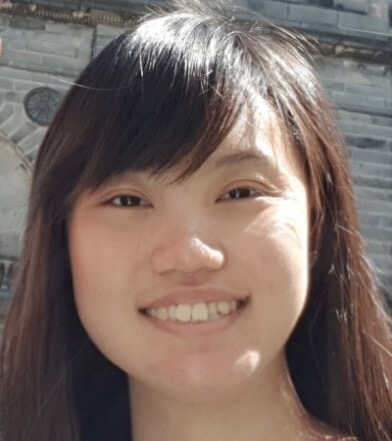
\includegraphics[height=0.1\textwidth]{photo.jpg}
        \hspace{20pt}
        \begin{minipage}[b]{0.83\textwidth}
            \texttt{unimpeded} is a re-usable library of posterior samples, nested sampling~\cite{skilling2006, 2022NRvMP...2...39A} runs and machine learning emulators across a grid of cosmological models for detecting cosmological tensions between datasets from the DiRAC allocation (DP192 \& 264). It serves as an analogous grid to the Planck Legacy Archive (PLA), but machine learning enhanced and expanded to enable not only parameter estimation (currently available with the MCMC chains on PLA), but also allowing cosmological model comparison and tension quantification. The emulators are implemented with piecewise normalising flows~\cite{2023arXiv230502930B} as part of the package \texttt{margarine}~\cite{2022arXiv220512841B, 2022arXiv220711457B}, though alternative density estimation methods can be used. The combination of nested sampling and density estimation allows us to obtain the same posterior distributions as one would have found from a full nested sampling run over all nuisance parameters, but many orders of magnitude faster. This allows users to use the existing results of cosmological analyses without the need to re-run on supercomputers.

        \end{minipage}%
        %\hspace{20pt}
        %
\includegraphics[height=0.09\textwidth]{kicc.png}

    }
\begin{columns}
    %\column{0.75}
    \column{0.5}
    
    \block{The three pillars of Bayesian inference}{%
        \begin{minipage}{0.22\textwidth}
            \innerblock{Parameter Estimation}{%
                What do the data tell us about the parameters of a model?
                e.g. the size or age of a $\Lambda$CDM universe
                \[ \C[0]{\text{Posterior}} = \frac{\C[2]{\text{Likelihood}} \times\C[1]{\text{Prior}}}{\C[3]{\text{Evidence}}}. \]
            }
        \end{minipage}\hfill%
        \begin{minipage}{0.22\textwidth}
            \innerblock{Model Comparison}{%
                How much do the data support a given model? e.g. $\Lambda$CDM vs a dynamic dark energy cosmology
                \[ \C[4]{\text{Posterior}} = \frac{\C[3]{\text{Evidence}} \times\C[5]{\text{Prior}}}{\C[6]{\text{Normalisation}}}.\]
            }
        \end{minipage}\hfill
        
        \vspace{10pt}
        \begin{minipage}{0.19\textwidth}
            \innerblock{Tension quantification}{%
                Do different datasets make consistent predictions from the same model? e.g. Hubble $H_{\mathrm{0}}$ tension from CMB vs Type 1A supernovae data
            \[ \mathcal{R} = \frac{\C[3]{\mathcal{Z}}_{AB}}{\C[3]{\mathcal{Z}}_A\C[3]{\mathcal{Z}}_\mathcal{B}}, \] 
            \[
                %\begin{aligned} \log\mathcal{S} = \av[{\C[0]{\mathcal{P}}_{AB}}]{\C[2]{\log\mathcal{L}}_{AB}}&\\
                    %-\av[{\C[0]{\mathcal{P}}_{A}}]{\C[2]{\log\mathcal{L}}_{A}}&\\
                    %-\av[{\C[0]{\mathcal{P}}_{B}}]{\C[2]{\log\mathcal{L}}_{B}}&
                %\end{aligned}
            \]
            }
        \end{minipage}\hfill
        \begin{minipage}[]{0.25\textwidth}
            Model comparison and tension quantification have become increasingly relevant in recently years because of anomalies, e.g. $H_{\mathrm{0}}$ and $\sigma_8$ tension. Although MCMC chains (currently available on PLA grids) may be used for parameter estimation, model comparison and tension quantification are far more computationally expensive, so more specialist tools like nested sampling are required.
        \end{minipage}
        
    }
%\end{columns}
%\begin{columns}
    %\column{0.5}
    \block{Available Models \& Data}{%
        \begin{minipage}{0.23\textwidth}
            \texttt{unimpeded} provides a systematic coverage of cosmological models, datasets and their pairwise comparisons. It will be expanded as new datasets and models become available, e.g. ACT, SPT, DESI, DESY5, Union, Patheon+,.... Requests for new datasets are welcome!
            
            
        \end{minipage}\hfill
        \begin{minipage}{0.21\textwidth}
            \innerblock{Cosmological datasets}{%
               \begin{itemize}
                   \item CMB:(Plik, Camspec, NPIPE, BICEP) $\pm$ CMB lensing
                   \item BAO:SDSS, BOSS, eBOSS, Ly$\alpha$
                   \item SNe: Pantheon, SH0ES
                   \item WL: DESY1
                    %\item Planck 2018 CamSpec 
                    %\item Planck 2018 CamSpec no lens
                    %\item Planck 2018 plik
                    %\item Planck 2018 plik no lens
                    %\item BAO SDSS DR16
                    %\item BICEP/Keck 2018
                    %\item DES year 1
                    %\item Pantheon SN
                \end{itemize} 
            }
        \end{minipage}\hfill
        \vspace{10pt}
        \innerblock{Cosmological models}{%
                \begin{itemize}
                    \item $\Lambda\mathrm{CDM}:H_{\mathrm{0}},\tau_{\mathrm{reio}},\Omega_{\mathrm{b}}h^2,\Omega_{\mathrm{c}}h^2,A_{\mathrm{s}},n_{s}$
                    \item $K\Lambda\mathrm{CDM}:\Lambda\mathrm{CDM}+\Omega_{K}$ (varying curvature)
                    \item $N\Lambda\mathrm{CDM}:$ Varying $N_\mathrm{eff}$ and total mass of 3 degenerate $\nu$'s
                    \item $n\Lambda\mathrm{CDM}:$ Varying total mass of 3 degenerate $\nu$'s with $N_\mathrm{eff}$=3.044
                    \item $m\Lambda\mathrm{CDM}:$ Varying $N_\mathrm{eff}$ with two massless $\nu$ and one with $m$=0.06
                    %\item $N\Lambda\mathrm{CDM}:\Lambda\mathrm{CDM}+N_\mathrm{eff}$ (varying effective number of relativistic species)  
                    \item $\mathrm{n_{run}}\Lambda\mathrm{CDM}:\Lambda\mathrm{CDM}+\mathrm{n_{run}}$ (running of spectral index $dn_\mathrm{s}/d\ln k$)
                    %\item $m\Lambda\mathrm{CDM}:$ magnetised $\Lambda\mathrm{CDM}$
                    \item $w\mathrm{CDM}:\Lambda\mathrm{CDM}+w$ (constant cosmological equation of state)
                    \item $w_0w_\mathrm{a}\Lambda\mathrm{CDM}:\Lambda\mathrm{CDM}+w_0+w_\mathrm{a}$ (varying dark energy equation of state, CLP)
                    \item $r\Lambda\mathrm{CDM}: \Lambda\mathrm{CDM}+r$ (varying scalar-to-tensor ratio)
                \end{itemize}
            }
       
    }

    \block{Results - Emulators}{%
        \begin{minipage}[]{0.21\textwidth}
            \texttt{unimpeded} provides a library of trained bijectors to be used as priors or emulators~\cite{2021MNRAS.505L..95A} or nuisance marginalised likelihoods~\cite{2022arXiv220711457B}. Piecewise normalising flows are used with \texttt{margarine} to model complex probability densities through bijective transformations between a base distribution and the target distribution. Density estimators, such as Kernel Density Estimators~\cite{parzen1962estimation, Rosenblatt1956} and Masked Autoregressive Flows~\cite{2017arXiv170507057P} are used to rapidly calculate reliable and reusable marginal probability densities and marginal Bayesian summary statistics for key signal or cosmological parameters.
        \end{minipage}\hfill
        \begin{minipage}[]{0.23\textwidth}
            %\centering
            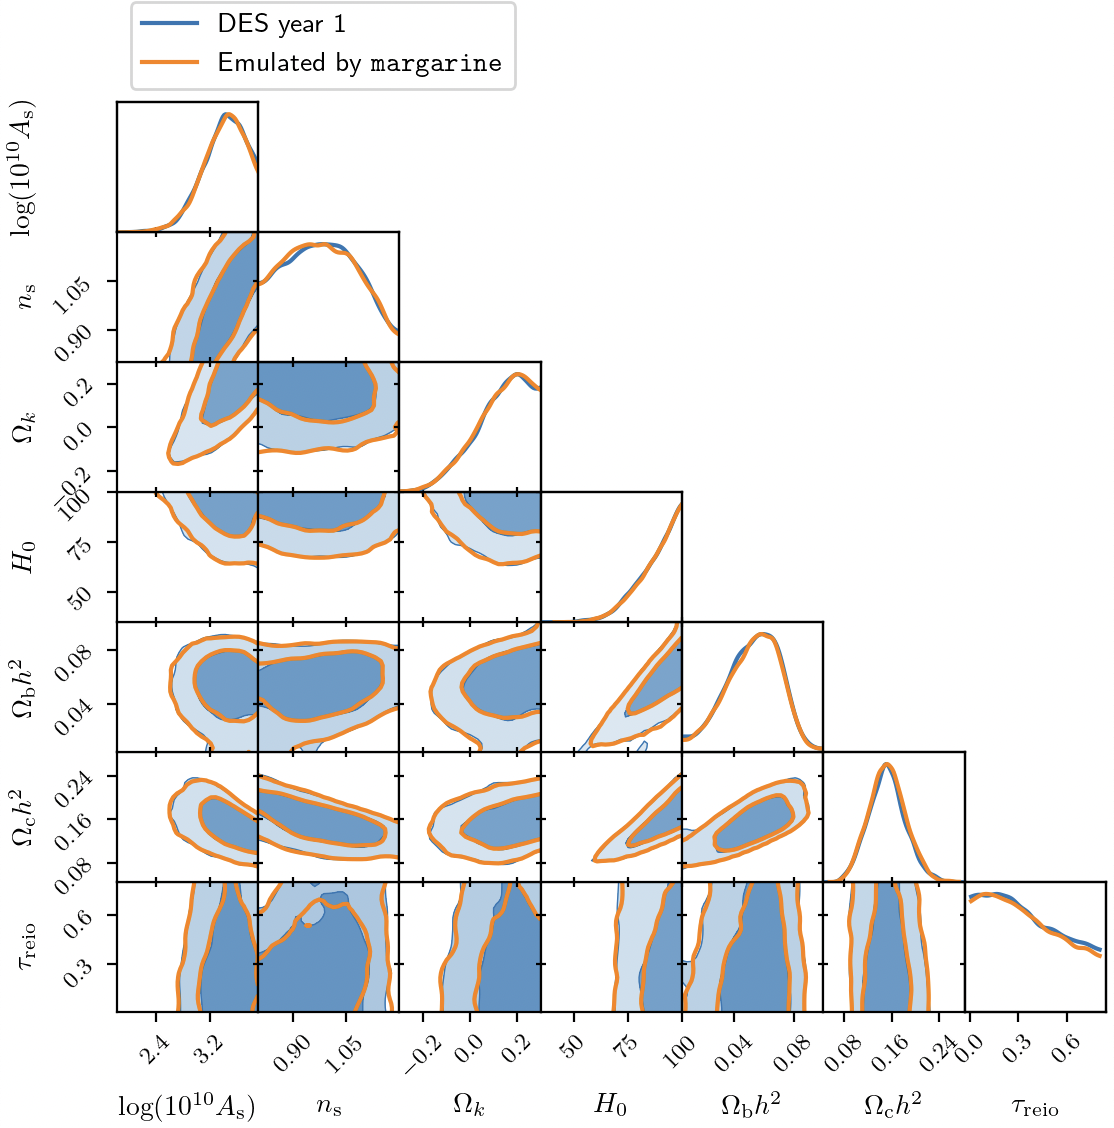
\includegraphics[width=\textwidth]{emulators_4.png}         
        \end{minipage}\hfill
         This enables the access to the nuisance-free likelihood functions, which greatly reduces computational cost in combining parameters constraints from different datasets. It allows users to use a real ’planck prior’ rather than a Gaussian approximation for future cosmological analyses. Here is an example of the DES year 1 dataset (blue filled contours) emulated by \texttt{margarine} (orange line) using nested sampling chains, with a p-value of 0.752.
    }

    \column{0.5} % This line decides when the second line begins

    \block{Using \texttt{unimpeded}}{%
        \texttt{unimpeded} is a Python tool for seamlessly downloading and cacheing chains (API in 'alpha'). It provides both MCMC and nested sampling chains. Data are stored on \texttt{zenodo}, with hdf5 storage for fast and reliable download and storage. \texttt{unimpeded} is a pip-installable package.
        %\coloredbox{\begin{center}\texttt{pip install unimpeded}\end{center}}
        \begin{tcolorbox}[colback=white,colframe=black,varwidth=\linewidth]
        \texttt{pip install unimpeded}
        \end{tcolorbox}
        To access any combination of these models and datasets (also the pairwise combinations of datasets, e.g. Planck 2018 CamSpec+DES year 1), simply call the function \texttt{unimpeded.get(data, model, method)} and specify the dataset, model and sampling method (ns = nested sampling or mcmc = Metropolis–Hastings MCMC mthods).
        %\coloredbox{\texttt{samples = unimpeded.get(data='planck\_2018\_CamSpec', model='lcdm', method='ns')}
        
        \begin{tcolorbox}[colback=white,colframe=black,varwidth=\linewidth]
        \texttt{samples = unimpeded.get(data='planck\_2018\_CamSpec', model='lcdm', method='ns')}
        \end{tcolorbox}
        \vspace{-15pt}
        
        
    }

    \block{Samplers}{%
        Samples are the fundamental building block of numerical Bayesian inference, encapsulating high-dimensional posterior probability distributions. The samplers used in \texttt{unimpeded} are Metropolis Hastings MCMC and Nested Sampling, using \texttt{Cobaya}~\cite{2021JCAP...05..057T}.
        %\vspace{-15pt}
        \begin{minipage}[]{0.22\textwidth}
            \innerblock{Metropolis–Hastings MCMC}{%
                \begin{minipage}[]{.5\textwidth}
                    \begin{itemize}
                        \setlength\itemsep{1.37em}
                        \item Single ``walker''
                        \item Explores posterior
                        \item Fast, if proposal matrix is tuned
                    %\item Channel capacity optimised for generating posterior samples
                \end{itemize}
                \end{minipage}
                \begin{minipage}[]{0.22\textwidth}
                    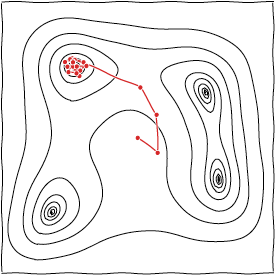
\includegraphics[height=2\textwidth]{mcmc.png}
                \end{minipage}
                \begin{itemize}
                    \item Parameter estimation, suspiciousness calculation
                    \item Channel capacity optimised for generating posterior samples
                \end{itemize}
                %\centering
                
                %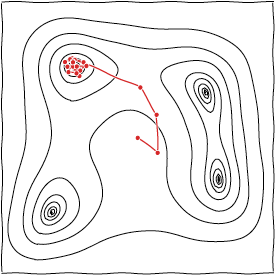
\includegraphics[height=0.4\textwidth]{mcmc}
            }
        \end{minipage}\hfill
        \begin{minipage}[]{0.22\textwidth}
            \innerblock{Nested Sampling}{%
                \begin{minipage}[]{.5\textwidth}
                    \begin{itemize}
                        %\item Parameter estimation, model comparison, tension quantification
                        \item Ensemble of ``live points''
                        \item Scans from prior to peak of likelihood
                        \item Slower, no tuning required
                    %\item Channel capacity optimised for computing partition function
                    \end{itemize}
                    \end{minipage}
                    \begin{minipage}[]{0.22\textwidth}
                        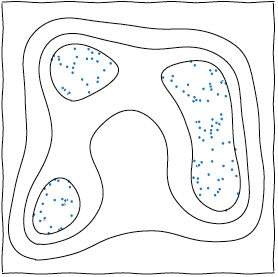
\includegraphics[height=2\textwidth]{ns}
                    \end{minipage}
                    \begin{itemize}
                        \item Parameter estimation, model comparison, tension quantification
                        \item Channel capacity optimised for computing partition function
                    \end{itemize}
            }
        \end{minipage}
        %\begin{tikzfigure}[Metropolis–Hastings MCMC mthods (left) and Nested Sampling (right).]
        %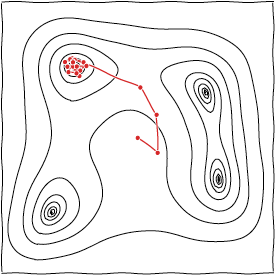
\includegraphics[height=0.13\textwidth]{mcmc}
        %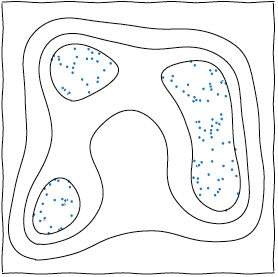
\includegraphics[height=0.13\textwidth]{ns}
        %\end{tikzfigure}
        \vspace{0.5em}
    
    }    
    

    


    \block{Preliminary Results - Tension Statistics}{%
        \begin{minipage}[]{0.17\textwidth}
            \texttt{unimpeded} acts as a tool for convenient and systematic measurement of tension statistics, and quantifying the Bayesian degree of confidence in comparing and combining datasets across different models. Available tension statistics include the $p$-value, $R$ statistics~\cite{Marshall2006}, the suspiciousness~\cite{Handley2019}, the information ratio from the Kullback-Leibler divergences and the Bayesian model dimensionality. Here is an example of one of the tension statistics ($\log R$) compared between 10 pairwise datasets across 9 cosmological models.
        \end{minipage}\hfill
        \begin{minipage}[]{0.29\textwidth}
            \centering
            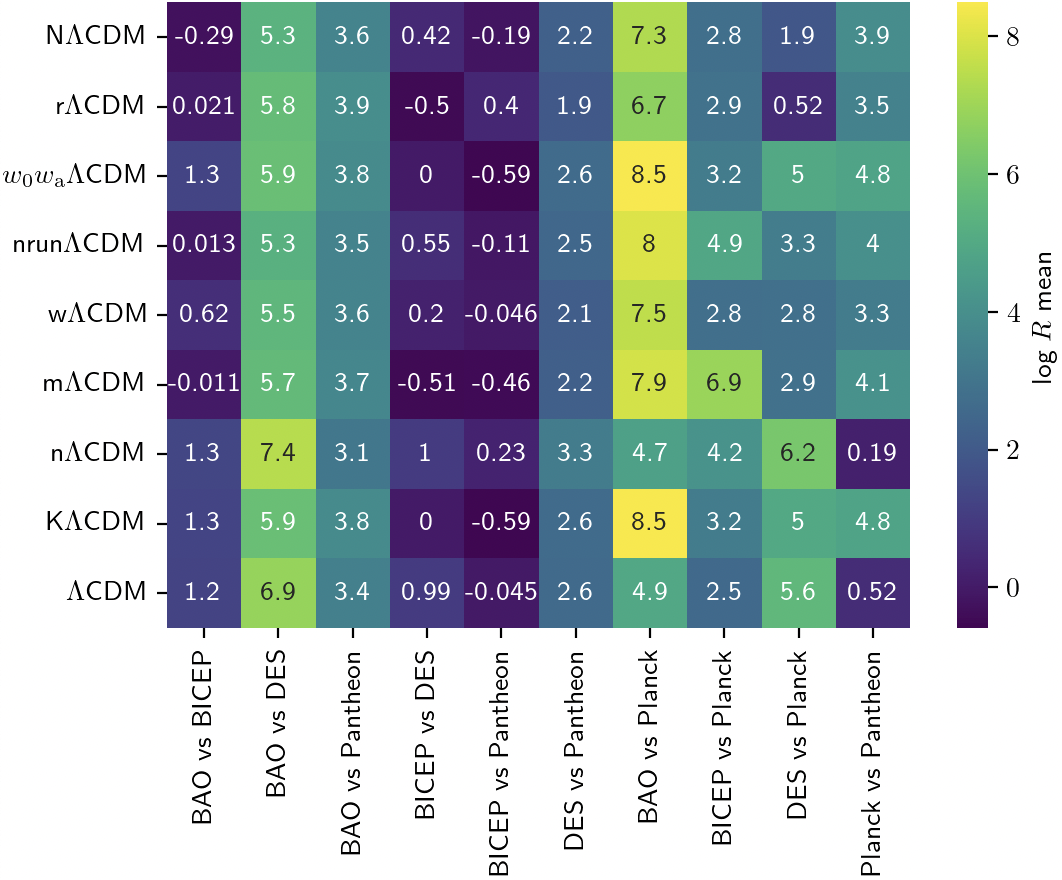
\includegraphics[width=\textwidth]{tension_2.png}
        \end{minipage}\hfill
    }



    \renewcommand{\section}[2]{}%
    \block{References}{%
        \begin{minipage}[b]{0.35\textwidth}
            \bibliographystyle{unsrt}
            \tiny
            This work was performed using the Cambridge Service for Data Driven Discovery (CSD3), part of which is operated by the University of Cambridge Research Computing on behalf of the STFC DiRAC HPC Facility (www.dirac.ac.uk). The DiRAC component of CSD3 was funded by BEIS capital funding via STFC capital grants ST/P002307/1 and ST/R002452/1 and STFC operations grant ST/R00689X/1.  DiRAC is part of the National e-Infrastructure.
            \bibliography{template_poster}
        \end{minipage}%
        \begin{minipage}[b]{0.14\textwidth}
            \hspace{90pt}
\includegraphics[width=0.35\textwidth]{QR_unimpeded_github.jpg}
            \vspace{30pt}
            
            \hspace{90pt}
\includegraphics[width=0.35\textwidth]{QR_poster.jpg}
        \end{minipage}%
        
    }

    \note[targetoffsetx=0.16\textwidth,targetoffsety=0.04\textwidth, connection,angle=135,radius=0.08\textwidth]{Github repository for \texttt{unimpeded} (top) and this poster (bottom).}
\end{columns}
\end{document}
